\chapter{Implementation and Testing}

This chapter focuses on the implementation stage of this project and discusses the development of the artefact's codebase; the development of this project is dissected into its respected categories, such as each significant chunks of code and overall testing. As stated in section 1, the project will form an executable deliverable which is expected to meet the requirements outlined in \autoref{section:FunctionalRequirements} and \autoref{section:NonFunctionalRequirements} which forms the Minimum Viable Product (MVP) until the final production release. The release of the final deliverable will handled in a staged environment to be assessed.

\section{Linking to Methodology}

This project was developed in an agile manner with continuous development as seen in \autoref{fig:CRISP-DM}, it had one major iteration to which adaptations built into the existing codebase; if test features were needed, a separate git branch was created as insurance the existing (working) code was not affected. The implementation phase is broken down into two key sections as this allows the developer to assess where or not the methodology is functioning as desired with their chosen tech-stack.

\section{Elected Programming Environment}

\subsection{Development Environment}

This project has made use of popular development environments with their own intended purpose:
\begin{itemize}
    \item \textbf{\textit{PyCharm:}} for general development.
    \item \textbf{\textit{Jupyter NoteBooks:}} for data organisation and visualization.
    \item \textbf{\textit{Kaggle NoteBooks}} for open-source testing and comparison.
\end{itemize}

\subsection{Language Choice and Justification}

There are more appropriate languages to consider for this project as the nature is how differing theory implementations affect performance and accuracy; C++ was considered at the beginning of this project due to its performance and execution speeds, popular machine learning libraries are written in C++ such as TensorFlow and ported to Python with the use of Cython. However, the learning curve for writing machine learning in C++ is a lot steeper than in Python to which Python was the chosen language for ease of use and development time.

As the artefact relies on programming knowledge, it was essential to pick a language the developer is comfortable writing in as learning a language for a specific use may have required dedicating too much time, especially with time-management overhead. This was beneficial as the developer has previous experience with Python and is relatively fluent.

As stated above, many a data mining \& analytics and machine learning libraries are written for or in Python which also increases the ease of use for project development with specific traits, such as NLP with ML. This project's interests are heavily backed with open-source development of Python libraries which ensure the imports are relatively low costing and the codebases work as efficiently as possible for a given task. This makes Python a well suited language for machine learning projects and is almost the goto language for data-science related tasks. \newpage

\subsection{Language libraries and Justification}

\begin{itemize}
    \item \textbf{\textit{Numpy:}} Data-Science library.
    \item \textbf{\textit{NLTK:}} Natural Language ToolKit for Python
    \item \textbf{\textit{Pandas:}} Popular Python Library for data-science, particularly, data manipulation and formatting.
    \item \textbf{\textit{Mathplotlib:}} Popular Python library for data visualization.
\end{itemize}


\section{Data Preparation and Parsing}

Firstly, the CSV sample data file needs to be cleaned; as the sample data is relatively a small dataset, it can be cleaned manually by simply deleting the unnecessary column headers and values. This was completed within Microsoft Excel by the developer.

Within \autoref{sub:C5Preprocessing}, it states four different data preprocessing methods will be applied, the implementation of those methods are as follows, starting with the removal of punctuation and English stop words.

\begin{figure}[H]
    \centering
    \includegraphics[width=\textwidth]{figures/chapter-6/data_preprocess.png}
    \caption[Code for punctuation and stopword removal]{Code for punctuation and stopword removal.
    \label{fig:data_preprocess}}
\end{figure}

\newpage

To remove colinear units and missing values, it is possible to use two pandas functions delete duplicate with specified parameters and is null for empty items, these functions can be called when reading an object, in this case read csv. Calling these functions at the same time does not affect computational cost.

\begin{figure}[H]
    \centering
    \includegraphics[width=0.9\textwidth]{figures/chapter-6/parse_sample.png}
    \caption[Code for colinear and missing values]{Code for colinear and missing values.
    \label{fig:parse_sample}}
\end{figure}

\subsection{Parsing Multiple Student Feedback Datasets}

The network's architecture allows for multiple data samples to be listed as sample input, this is useful as institutions may have multiple sources of training data. At the base level, a simple static file merged into a panda's dataframe will allows for all values across multiple datasets to be read simultaneously and propagated through the hidden layer. As long as the datasets are cleaned beforehand, the model will weigh and evaluative each datum entry.

\begin{figure}[H]
    \centering
    \includegraphics[width=0.9\textwidth]{figures/chapter-6/parse_multiple_dataframes.png}
    \caption[Statically parse multiple dataset]{Statically parse multiple dataset.
    \label{fig:parse_multiple_dataframes}}
\end{figure}

\section{Network Architecture and Hyper-Parameters}

When designing the model's architecture in \autoref{sub:Word2VecSkipGram}, it was apparent the model could make use of environment variables to classify aspects of the model's training phase; the network uses seven env variables as hyper-parameters, these parameters are:

\begin{figure}[H]
    \centering
    \includegraphics[width=\textwidth]{figures/chapter-6/network_architecture.png}
    \caption[Hyper-parameters for network]{Hyper-parameters for network.
    \label{fig:network_Hyper_parameters}}
\end{figure}

Each variable is representative of the work outlined in \autoref{sub:Word2VecSkipGram}, where:

\begin{itemize}
    \item \textbf{\textit{word dimension:}} the number of columns in the first matrix.
    \item \textbf{\textit{panel size:}} size of a vector's space.
    \item \textbf{\textit{count:}} word count in an embedding
    \item \textbf{\textit{passing epoch value:}} how many epochs the model will have, passing through nodes.
    \item \textbf{\textit{ne sample:}} negative sampling count for a word vector.
    \item \textbf{\textit{learning rate:}} variable to swap the impact of learning.
    \item \textbf{\textit{network seed:}} using a specific seed to account for reproducibility.
\end{itemize}

\section{Network Class}

As the network's environment variables have been defined, this allows a secondary use as hyper-parameters which will need to be initialised within the class name and initialisation functions.

\begin{figure}[H]
    \centering
    \includegraphics[width=\textwidth]{figures/chapter-6/word2vecclass.png}
    \caption[Class structure for the Word2Vec SkipGram Model]{Class structure for the Word2Vec SkipGram Model.
    \label{fig:word2vec_class}}
\end{figure}

Pre-defining commonly used global variables within the class scope allows for the model to create presumptions on how the data being feed into it must be handled, specifically concerning the two matrices used as Python's array does not function as desired here to which the use of numpy's 2d array is shown.

\section{One-Hot Encoding}

oene hot \autoref{sub:Word2VecOneHotEncoding}

\begin{figure}[H]
    \centering
    \includegraphics[width=\textwidth]{figures/chapter-6/OneHotEncoding.png}
    \caption[Coding function for encoding word units as a One-Hot vector]{Coding function for encoding word units as a One-Hot vector.
    \label{fig:onehot_encoding}}
\end{figure}

\section{Forward Propagation}

f p \autoref{sub:Word2VecForwardPropagation}

\begin{figure}[H]
    \centering
    \includegraphics[width=\textwidth]{figures/chapter-6/forwardpropagation.png}
    \caption[Coding function for forward propagation]{Coding function for forward propagation.
    \label{fig:forwardpropagation}}
\end{figure}

\subsection{Softmax Function}



\begin{figure}[H]
    \centering
    \includegraphics[width=\textwidth]{figures/chapter-6/softmaxfunction.png}
    \caption[Softmax function for forward error parsing]{Softmax function for forward error parsing.
    \label{fig:softmaxfunction}}
\end{figure}

\section{Backward Propagation}

b p \autoref{sub:Word2VecBackardPropagation}

\begin{figure}[H]
    \centering
    \includegraphics[width=\textwidth]{figures/chapter-6/backwardpropagation.png}
    \caption[Coding function for backward propagation]{Coding function for backward propagation.
    \label{fig:backwardpropagation}}
\end{figure}

\section{Network Training}

\begin{figure}[H]
    \centering
    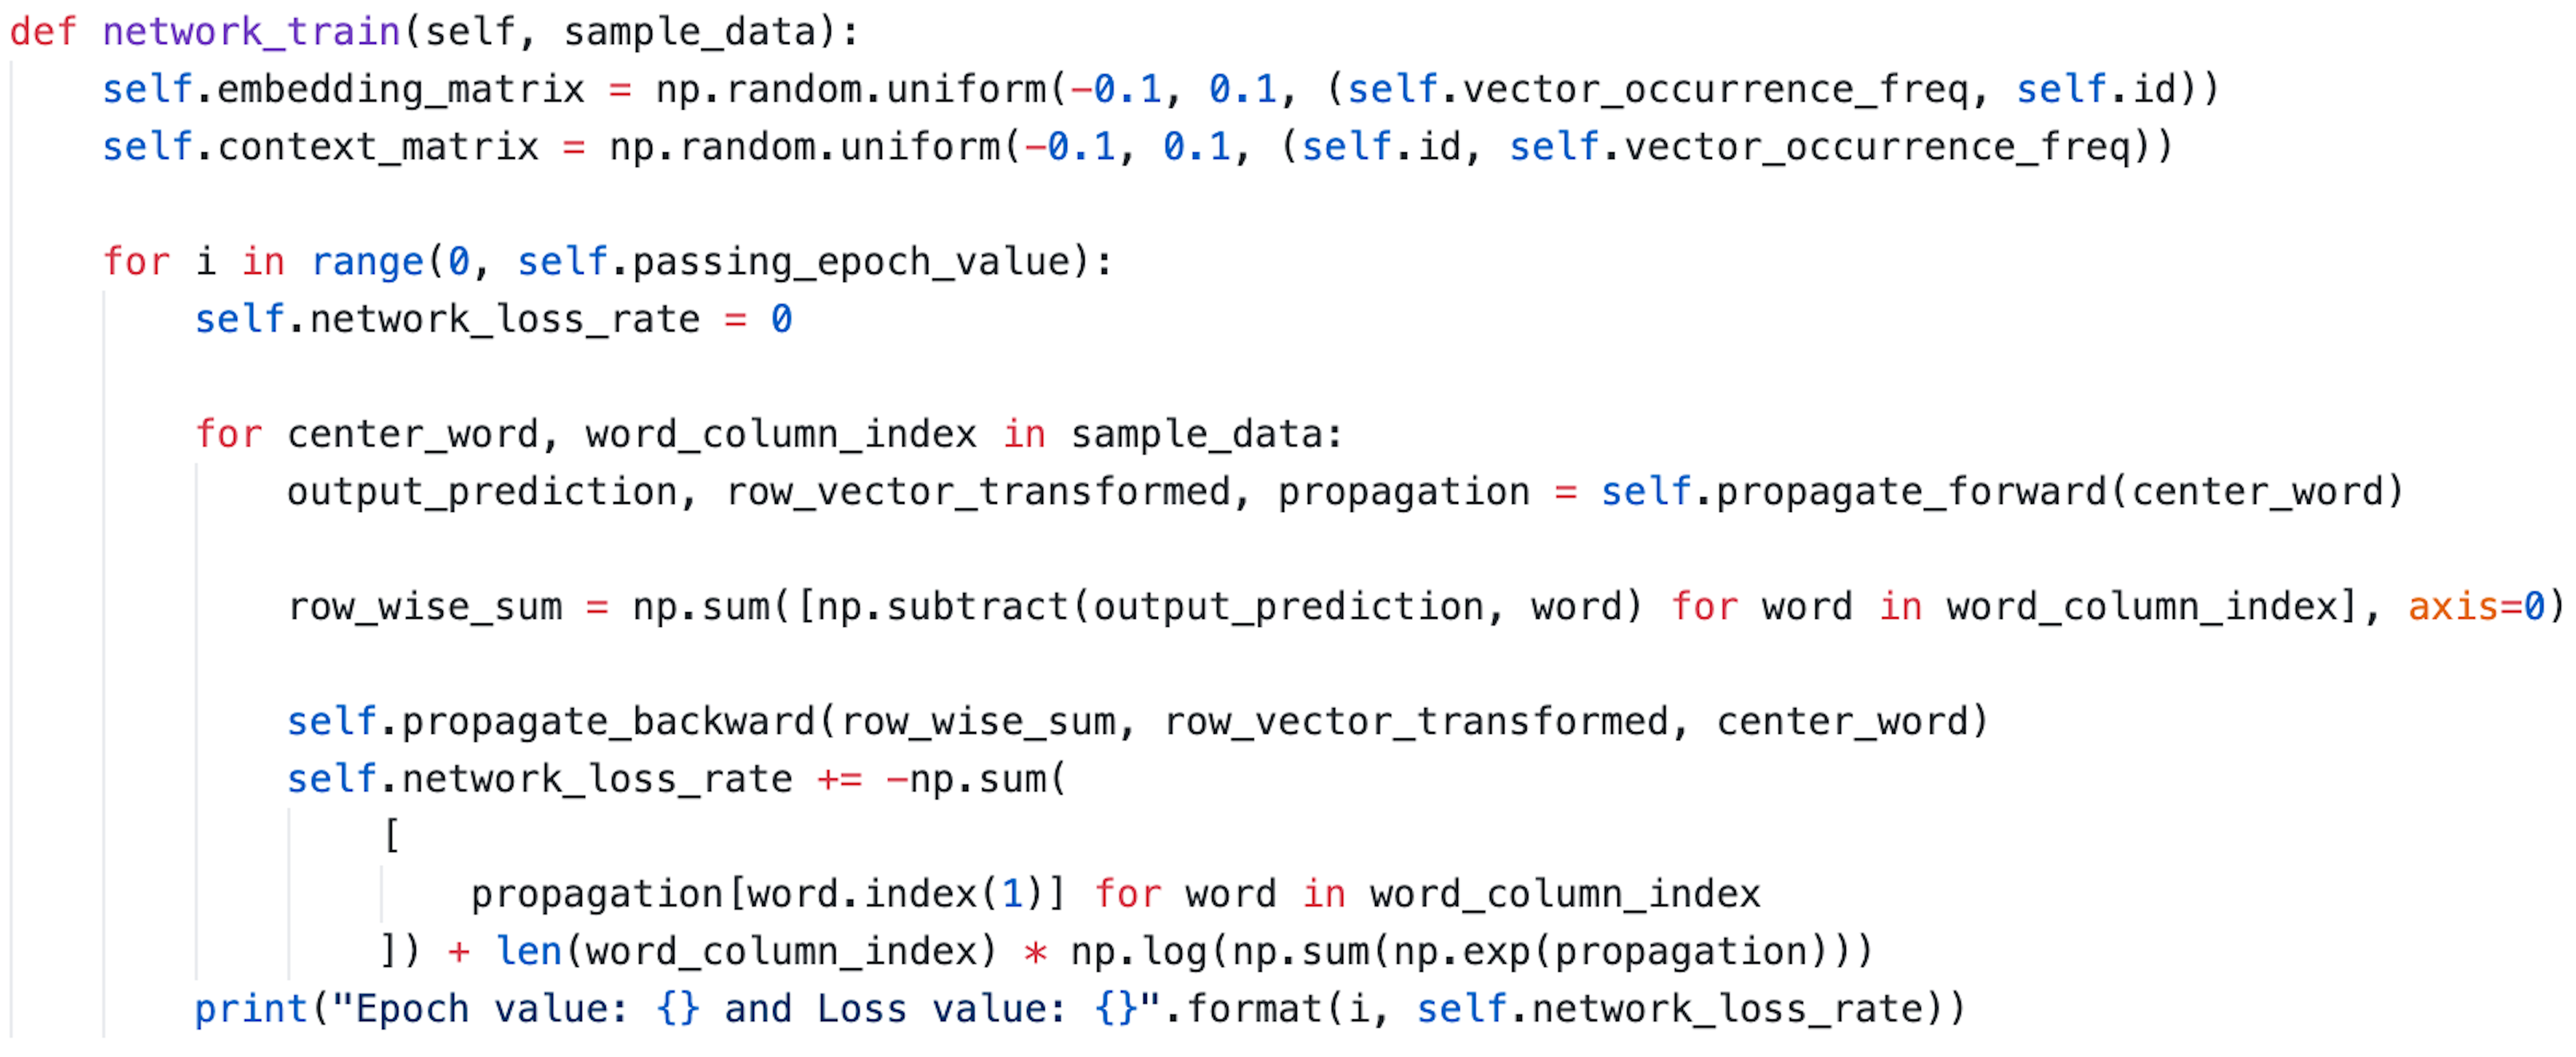
\includegraphics[width=\textwidth]{figures/chapter-6/network_train.png}
    \caption[Training of network]{Training of network.
    \label{fig:network_train}}
\end{figure}

The code snippet displayed in \autoref{fig:network_train}, returns the following data; at the lowest level, the fundamental model used epoch values to represent the passing through the hidden layer to which calculate data loss via the loss function specified in \autoref{fig:softmaxfunction} and \autoref{eq:C5ErrorCalc}.

\begin{figure}[H]
    \centering
    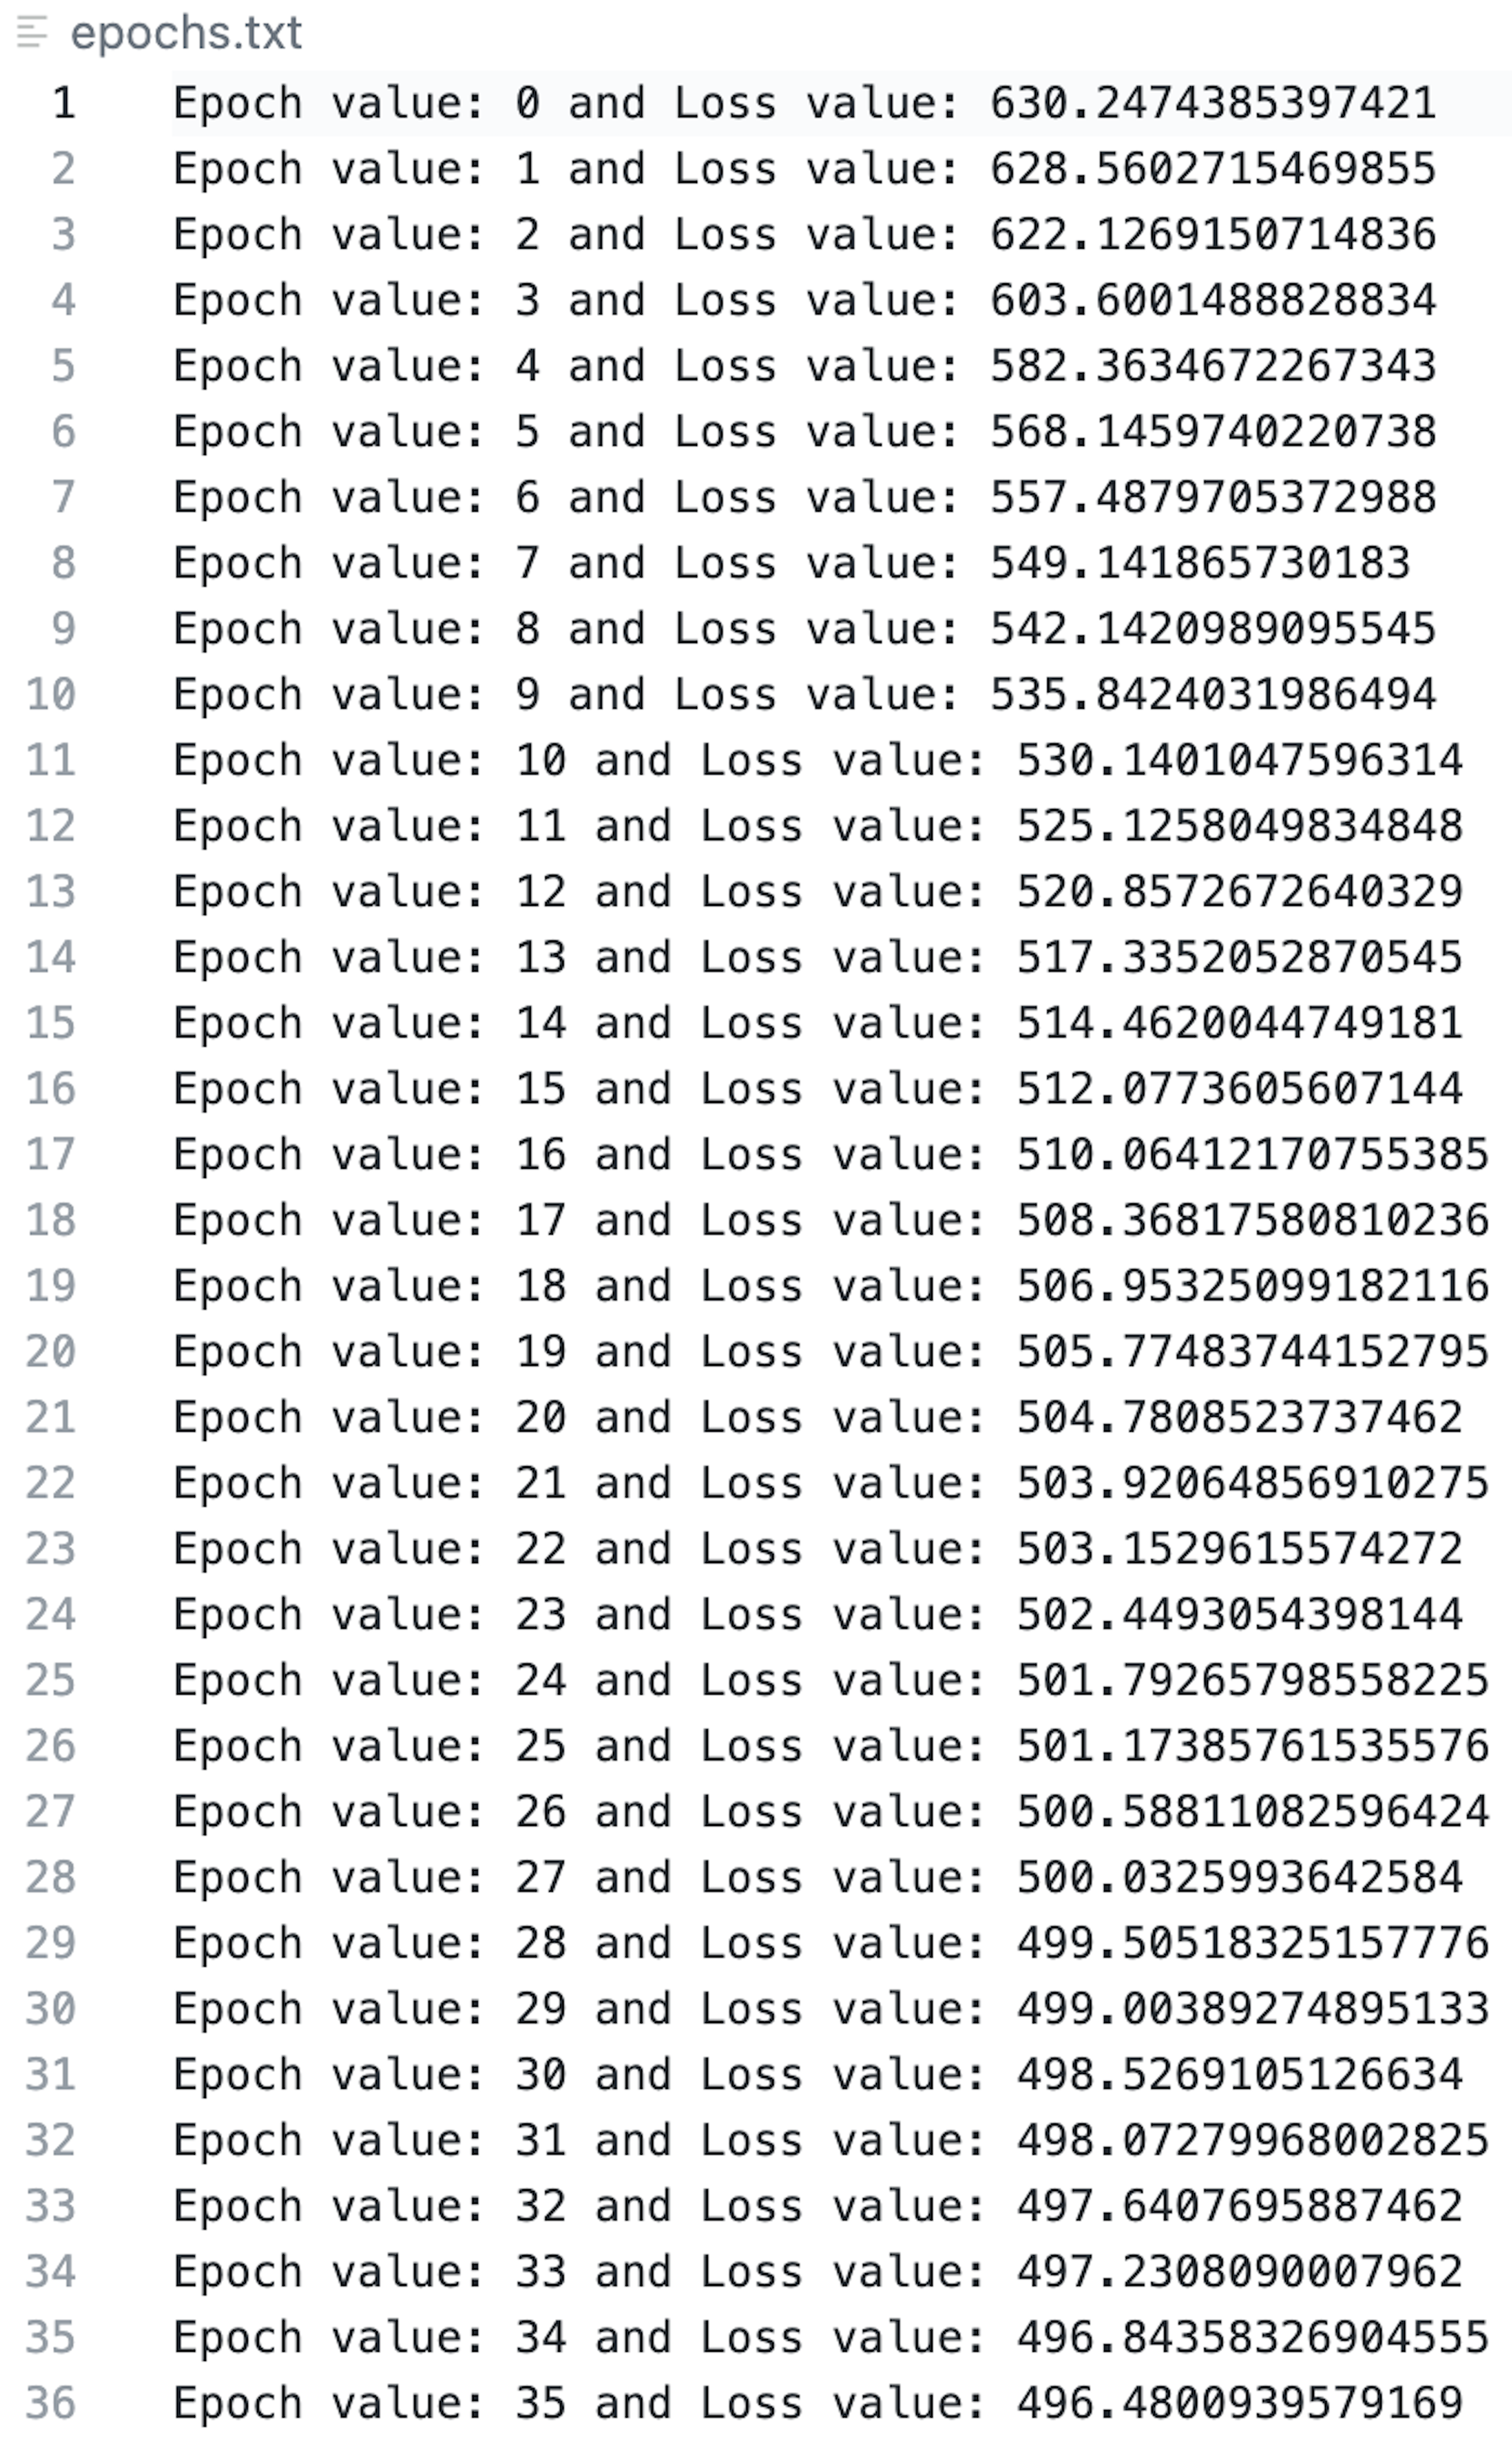
\includegraphics[]{figures/chapter-6/Training_Multiple_DataSets.png}
    \caption[Training network on multiple sets of student feedback]{Training network on multiple sets of student feedback.
    \label{fig:Training_Multiple_DataSets}}
\end{figure}

\subsection{Graphing with Mathplotlib}

As displayed in \autoref{fig:Training_Multiple_DataSets}, it is clear the model's training is successful as with each passing epoch, the loss value decreases, finding the optimal number of epochs simply entailed increase by a factor of 1 until the loss value did not hold a constant pattren. The figures below show both of the network's matracies $W$ and $W'$ in relation to each passing epoch; with each iteration the word embeddings got higher weighted and lower in regards to word vector, whereas word context was evenly spread at a strong impact value. This shows that the model is a sucess for training student feedback and can be a viable training model for text and text classification methods.

\begin{figure}[H]
    \includegraphics[width=0.49\columnwidth]{figures/chapter-6/epoch1.png}
    \includegraphics[width=0.49\columnwidth]{figures/chapter-6/epoch58.png}
    % For long captions include a short version for the List of Figures/Tables sections in square brackets as below.
    \caption[Epoch Evolutions for Network]{Epoch Evolutions for Network, displaying the embedding matrix (green) and context matrix (red)
    \label{fig:EpochEvolutions}}
\end{figure}

\section{Convert Word to Vector Value}
\begin{figure}[H]
    \centering
    \includegraphics[width=\textwidth]{figures/chapter-6/convertwordvector.png}
    \caption[Conversion of word to vector value]{Conversion of word to vector value.
    \label{fig:convertwordvector}}
\end{figure}

\section{Word Vector Sum}

\begin{figure}[H]
    \centering
    \includegraphics[width=\textwidth]{figures/chapter-6/wordvectorsum.png}
    \caption[The weighting of all word vectors]{The weighting of all word vectors.
    \label{fig:wordvectorsum}}
\end{figure}

\section{Word Sum}

\begin{figure}[H]
    \centering
    \includegraphics[width=\textwidth]{figures/chapter-6/wordsum.png}
    \caption[The weighting of all words]{The weighting of all words.
    \label{fig:wordsum}}
\end{figure}
